\section{Results}
\label{sec:results}

The primary experiment is the Class~A search for a drifting, unresolved
spectral carrier: \NWinA{} fine-channel windows toward \NSysClassA{}
systems, \EdrNWinA{} of which are channelised finely enough on the criterion
of \S\ref{sec:statistic} to tell a drifting carrier from a stationary one.
The Class~B search for an unresolved spectral excess is secondary
and carries no drift discrimination: \NWinB{} coarse windows. Together they
are the \NWindows{} windows of the primary census. No event
satisfied the confirmation criterion set out in \S\ref{sec:summary}. Depth
comes first below, then what the search found and how each finding was
disposed of.

\subsection{Sensitivity: the power at which a carrier would have crossed
the threshold} \label{sec:pninetysel}

\emph{The median system, on its best window, would have produced a threshold
crossing from a carrier of $\EirpNinetySysMedA$\,W.} Across the \NSysClassA{} systems those limits
run from $\EirpNinetySysLoA$ to $\EirpNinetySysHiA$\,W
(Fig.~\ref{fig:classasens}a), and \NSysEfifteen{} of the systems reach
$10^{15}$\,W. The median Class~A \emph{window} reaches
$\EirpNinetyWinMedA$\,W.
Over the \EdrNWinA{} windows in which the searched drift crosses a channel
(\S\ref{sec:statistic}) the search covers \EdrUnionGHz\,GHz toward
\EdrNSys{} systems, and their median system limit is \ScEdrMedPct{} per cent
\ScEdrMedSense{} than the figure above.

\emph{They are a recovery completeness of one epoch, and not a threshold.}
Artificial carriers were injected at a random sub-channel phase and a random
drift from each window's own grid, then recovered through the unchanged
pipeline; the power at which nine in ten come back is
$\mathrm{EIRP}_{90}$, the only sensitivity quoted here. It is measured
through the single-epoch trigger and the localisation at the stellar position
inside one execution block. It is therefore the power at which a
carrier would have produced a crossing and not the power at which one would
have been confirmed, because confirmation needs a second and separated epoch, which the archive
supplies for some systems and not others (\S\ref{sec:confirmability}). The \NCtrl-position spatial rank
decides nothing and is not charged against it either: charging it would cost
a further factor $\SensCostLike$, and in \SensNRingHiUnres{} bright-ring
windows it could not be met at any injected power (Fig.~\ref{fig:strata}).

\emph{Measured that way the completeness is one number for the class.} Nine
carriers in ten are recovered at $\EirpNinetyMultA\,P_{\rm trig}$, and the
sampling error of that pooled value is $\pm\SensBootPct$ per
cent, a statement about the class average and about no individual
window. It is a
total power set against a nominal threshold, $P_{\rm trig}$ being the bare
$\LtCommonSnr\sigma$ of the window itself. The loss a channel-confined
carrier suffers to the correlator's spectral response is carried by the
injected tones, so it sits inside the measured factor -- $\times\RpRespFac$
of it -- and is not applied to the result as well
(Appendix~\ref{app:conventions}). Every one of the \SensNInj{} directly
injected Class~A windows resolves a ninety per cent point of its own, and the
value does not depend on the brightness of its control ring: the
\SensNRingHi{} windows whose ring carries resolved emission -- a ring
brightness above $\SensRingRule\sigma$, which is where the dotted line of
Fig.~\ref{fig:strata} falls -- come back at
$\SensRingHi\,P_{\rm trig}$ against $\SensRingLo$ for the rest
(Fig.~\ref{fig:strata}). Class~B carries its own factor $\EirpNinetyMultB\,P_{\rm trig}$, which
sets the limits for Barnard's Star, Wolf~359 and Proxima. It is measured the
same way, from \SensNToneCoarse{} carriers injected into \SensNInjCoarse{}
coarse windows of \SensNInjCoarseBlock{} execution blocks.

Calibration of that factor is good to
$\times\SensFacLo$--$\times\SensFacHi$ (Table~\ref{tab:p90budget}), which is
an interval on the median and on the counts and not on any one window's
limit. The median system's limit above carries it -- $\TfMedCalLo$ to
$\TfMedCalHi$\,W -- so the second figure of that median is set by the
calibration and not by the depth of any observation.

\emph{Every limit quoted here is nominal in one respect: it excludes
atmospheric decorrelation.} An injected carrier is added to already
calibrated visibilities and so suffers none, whereas a real carrier does, and
the bias runs one way only. Measured block by block from the phase rms the
observatory records on each block's phase calibrator
\citep[\S\S10.4.11, 11.3.1]{ALMAHandbook}, through the standard phase-scatter
relation \citep[Eq.~3]{Richards2022}, it leaves the median limit optimistic
by \SensDecorPct{} per cent, and the median window above
\SensDecorHiGHz\,GHz by \SensDecorHiPct{} per cent.
\emph{That is why this term is stated and not
folded in}: the factors that are applied are available for every window
of the census, while this one is available for \SensDecorNBlk{} blocks of
\SensDecorNBlkTot{} and the rest are measurably the harder ones, so folding
it in where it is known would leave a set of limits that is neither corrected
nor uncorrected. Table~\ref{tab:persys} gives it system by system, measured
from the phase calibrator of a system's own block where the delivery exposes
one and imputed from the blocks matched to it in baseline length where it
does not (Appendix~\ref{app:persys}).

Three further factors act window by window and are divided out of the limits
above rather than quoted beside them: the primary-beam response at the star's
own offset from the pointing centre, the annual parallax the search's phase
centre omits, and the smearing of a carrier that sweeps within a channel
during one integration while an injected one does not.
Table~\ref{tab:p90budget} gives each with its range and its direction,
Appendix~\ref{app:conventions} the definitions and
Appendix~\ref{app:pbresp} the astrometric terms, and the released per-window
catalogue carries each window's own value. The beam response is evaluated on
the full width the observatory documents, at each window's own dish diameter
and centre frequency, which of the two widths available is the one that
follows a blocked circular aperture; that choice is the largest of the three
and moves no quoted limit by more than \BmModelMaxPct{} per cent.
\emph{The net bias on one window's limit is therefore of either sign.} In the
median window the injected profile's \InjShortPct{} per cent shortfall
against the exact channel response is the larger term and the quoted limit is
conservative by \NmNetConsPct{} per cent; at the ninetieth percentile of the
systems' own best windows the decorrelation is, and the limit is optimistic
by \NmNetOptPct{} per cent, rising to \NmNetOptMaxPct{} per cent for the most
affected system. Neither direction describes the sample, which is why
Table~\ref{tab:persys} gives the decorrelation system by system.

\emph{Carriers were injected directly into \SensNInj{} of the \NWinA{}
Class~A windows, \SensNInjPct{} per cent, and the result transferred to the
remaining \SensNTransfer. That transfer is the dominant caveat on everything
above.} The injected windows are the Class~A windows of execution blocks
drawn in a random order, balanced by band and array; they hold
\SensNCrossAch{} crossings against the \SensNCrossExp{} the population rate
predicts. \emph{The unit is the block and not the window}, because a block's
calibrated visibilities are what an injection campaign has to rebuild, so
band and array were fixed by the draw and the conditions that vary within a
block were compared with the population afterwards.

That comparison covers \RpNAxis{} properties -- channel width, integration
time, noise, control-ring brightness, the channels a carrier at the drift
ceiling crosses in one track, and the intra-integration retention -- and on
every one the injected windows span the central eight-tenths of the
population, five of them agreeing in the median to \RpCovOtherPct{} per cent.
The sixth, \RpCovWorstAxis, does not: the injected windows are
$\times\RpCovWorstRatio$ noisier, which follows from drawing whole blocks,
and it is also the property the measurement is built to be insensitive to,
each ladder being in units of its own window's threshold: splitting the
injected set at the median of each property in turn moves the ninety per cent
point by at most \RpFacShiftMax\,$P_{\rm trig}$ (Appendix~\ref{app:persys}).

A window that was not injected therefore carries an estimated
$\mathrm{EIRP}_{90}$. One dimensionless number per class is
carried across -- the ninety per cent point in units of the window's own trigger power
-- while the channel width, the noise, the integration time, the primary-beam
response, the parallax displacement and the intra-integration retention that
turn it into a power are each that window's own measurement.
Across the injected windows the ninety per cent point
ranges from $\times\SensIndivFacLo$ to $\times\SensIndivFacHi$ of the
adopted factor, with \NmDispNTenth{} of the \SensNInj{} lying within a tenth
of it. The upper end of that range is one window and not a typical error: the
second largest is $\times\NmDispSecond$. That dispersion, and not the calibration
interval above, is what one uninjected window's own limit is uncertain by.
Two bands and two channelisations of the survey hold no injected window at
all, \NgNExtrapWin{} windows between them, and \NgNExtrapSys{} systems take
their best window from one: \NgExtrapSys. Their completeness is carried
across a configuration boundary and not within one, and because no
injected window lies in those configurations the range just quoted is not an
empirical bound on it. The deepest limit in the survey is one of these.
The best window was itself injected into for \SmcNMeasSys{} of the
\NSysClassA{} systems, marked as measured in Table~\ref{tab:persys}; for the
other \SmcNEstSys{} the headline limit is an estimate carrying that
dispersion. Each of those six at its own measured
factor instead of the class average would move by at most \NmOwnDevPct{} per
cent, and over the population the estimate is not biased in a direction one
can name (Appendix~\ref{app:persys}).

\emph{A carrier that is not always radiating is penalised in proportion}: over
\DutyNTrial{} trials at duty cycles down to \DutyCycleMinPct{} per cent the
recovered amplitude followed the duty cycle to \DutyAttenDevPct{} per cent, so
a transmitter radiating a tenth of the time needs $\DutyPowFac\times$ the
power quoted above. Those trials carry no drift, so the joint drifting and
intermittent case is not measured here.

\begin{table*}
\centering
\scriptsize
\caption{What sets $\mathrm{EIRP}_{90}$, and in which direction. The
calibration interval applies to the class-average factor and so to any
statistic over many windows; the spread between windows is an observed
dispersion and is the statement about one window; the signed terms are biases
and are not folded into an error bar (\S\ref{sec:pninetysel}).}
\label{tab:p90budget}
\setlength{\tabcolsep}{2pt}
% GENERATED by sens_r11.py -- do not hand-edit.
\begin{tabular}{@{}l@{~~}r@{~~}>{\raggedright\arraybackslash}p{0.61\linewidth}@{}}
\hline
 & value & what it does to the limit \\
\hline
Class-average completeness & $\times3.03$ & nine carriers in ten recovered at this multiple of a window's own trigger power. \emph{Measured} in the 49 Class~A windows injected directly and \emph{estimated}, at this factor, in the other 356 \\
\hline
\multicolumn{3}{@{}l}{\emph{Uncertainty on that calibration} (per cent), combined in quadrature} \\
The factor itself & $\pm2$ & sampling error of the pooled value over the 49 injected windows \\
Absolute flux scale & $\pm\BudFlux$ & the observatory's own band-dependent specification (\BudFluxSource): \BudFluxSpec, weighted over this sample's bands \\
Distance and visibility scale & $\pm\BudDistVis$ & the Gaia parallaxes, which enter as $d^{2}$, and the block-to-block visibility scale \\
\emph{Combined} & $-11/+11$ & $\times0.89$--$\times1.11$ on the factor, and so on the median limit and on the system counts; $\pm\BudCombWorst$ for the \BudNHiWin{} Class~A windows in \BudHiBandWord~\BudHiBands, at \BudHiGHzList\,GHz \\
\hline
\multicolumn{3}{@{}l}{\emph{Spread between windows}. An observed dispersion, not an error bar.} \\
Window to window & $\times0.80$--$\times1.58$ & the 49 injected windows resolve 2.41--4.80\,$P_{\rm trig}$ individually, \NmDispNTenth{} of them within a tenth of the pooled value and the second largest at $\times\NmDispSecond$. This, and not the interval above, is what an estimated limit is uncertain by; it is wider, and it applies to \SmcNEstSys{} of the \NSysClassA{} systems \\
\hline
\multicolumn{3}{@{}l}{\emph{Applied}. Folded into every limit quoted, and so not combined with the above.} \\
Intra-integration smearing & $\times1.00$--$\times\SmcFacWorst$ & a carrier sweeps through part of a channel within one integration and the injected ones do not: $\eta_{\rm smear}$ at the drift that sets a ninety per cent point, from each window's own integration length where it is recorded (\SmcNMeas{} windows) and from the longest delivered anywhere where it is not (\SmcNBound) \\
Primary beam & $\times1.00$--$\times\NmBeamFacWorst$ & the star is not at the pointing centre, so each limit is divided by the response at its own offset, on the full width the observatory documents. Nothing in the median window; the \BmNAboveTenPct{} windows furthest off-axis carry the departure of that form from a blocked circular aperture, up to \BmModelMaxPct{} per cent, as a one-sided systematic \\
Annual parallax & $\times1.00$--$\times2.06$ & the phase centre omits it, so each limit is divided by the amplitude a compact source retains at its own displacement, a median \PxaLossMedPct\,per cent \\
\hline
\multicolumn{3}{@{}l}{\emph{Signed terms}. A bias is not an error bar and is not added to one.} \\
Channel response & $\times\RpRespFac$ & the share of a channel-confined carrier the peak channel keeps. Carried by the injections, so already inside the completeness above, which is this factor times a margin of $\times\RpMarginNinety$ over the nominal trigger \\
\quad its residual & $+\InjShortPct$ & the injected profile falls short of the exact response: \emph{conservative} \\
Decorrelation & $+0/+\SensDecorPct$ & measured block by block from the phase rms the observatory records on each block's phase calibrator, which an injected carrier does not suffer and a real one does: $+\SensDecorHiPct$ above \SensDecorHiGHz\,GHz, and more than $+\SensDecorTailLevelPct$ in \SensDecorTailPct{} per cent of windows \\
\hline
\end{tabular}

\end{table*}

\begin{figure}
\centering
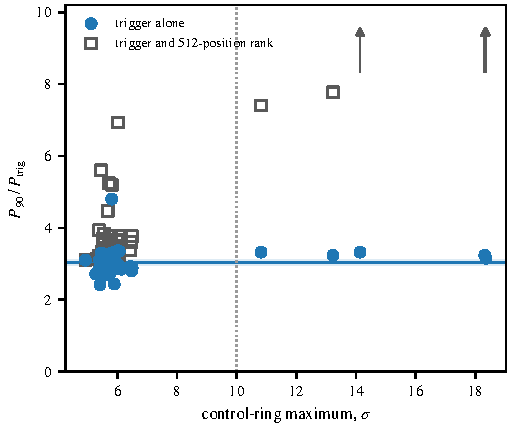
\includegraphics[width=\columnwidth]{figures/sens_ring.pdf}
%% ★ v4.26 (r25-captions): 9 printed lines -> R1 §7's limit of about six.
%% \S\ref{sec:pninetysel} above already carries every statement removed:
%% that the value does not depend on the ring's brightness, what charging
%% the rank would cost, and the bright-ring windows that cannot meet it at
%% any injected power -- the arrows.  \SensRingRule had this caption as its
%% only citation site, so the dotted line's threshold MOVED into that
%% paragraph rather than being dropped.
\caption{Why one completeness factor serves the whole class. The
\SensNInj{} directly injected Class~A windows at the power recovering nine
carriers in ten, each against its own \NCtrl-position ring maximum: no trend
with the ring. Filled, the criterion adopted here, pooled value as line and
band; open, the rank charged too, arrows where no power meets it; dotted, a
resolved ring.}
\label{fig:strata}
\end{figure}

\begin{figure*}
\centering
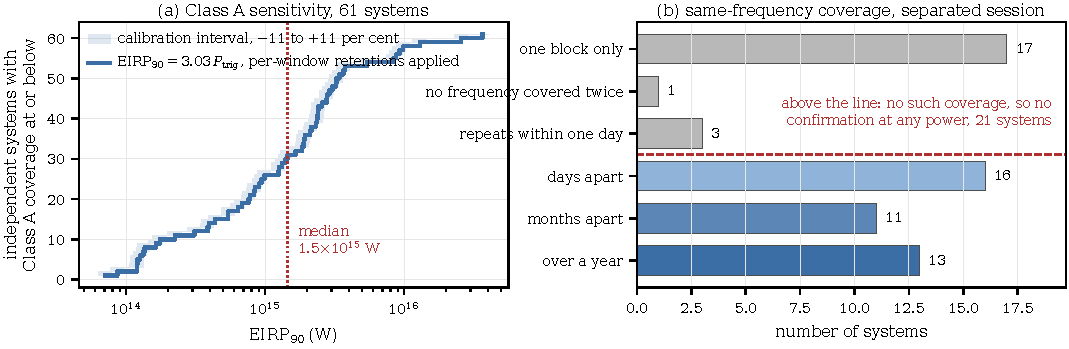
\includegraphics[width=\textwidth]{figures/classa_sensitivity.pdf}
%% ★ v4.26 (r25-captions): 9 printed lines -> R1 §7's limit of about six.
%% DELETED as said elsewhere and verified before deleting: "for an
%% accelerating carrier, confirmation further requires the repeat to fall at
%% a matching orbital phase" stands in Fig.~\ref{fig:confcov}'s caption AND in
%% \S\ref{sec:confirmability}; the grouping over "the primary census together
%% with every repeat block the recurrence test reads" is
%% \S\ref{sec:confirmability}'s own sentence; and the closing paragraph
%% re-states that section's opening line, "a sensitivity limit and a
%% confirmation limit are different statements", which is kept here in one
%% clause because it is what the figure is for.  No macro lost a site.
\caption{\textbf{The two completenesses of the carrier search, over the same
\NSysClassA{} systems}, which are separate statements and neither of which
follows from the other (\S\ref{sec:confirmability}).
\emph{(a)}~Single-epoch trigger completeness: the cumulative number of
systems whose best window reaches a given $\mathrm{EIRP}_{90}$, each
window's own retentions applied and atmospheric decorrelation excluded
(Table~\ref{tab:p90budget}, whose calibration interval is the shaded band).
\emph{(b)}~Systems with same-frequency coverage in a separated session,
which no amount of power buys, grouped by the longest separation between two
such sessions. \textbf{Left of the dashed line, \ZcNoRepSys{} systems have
no such pair, and for them confirmation was not possible at any sensitivity
in panel~(a)}.}
\label{fig:classasens}
\end{figure*}

\subsection{The nearest stars: Barnard's Star and Wolf~359}
\label{sec:barnardswolf}

Barnard's Star is the second-nearest stellar system and Wolf~359 the third if
brown dwarfs are excluded, and to our knowledge these are the first millimetre
or submillimetre technosignature limits for either; radio searches of
the nearest stars have worked at centimetre wavelengths \citep{Enriquez2017,
Price2020, Margot2023}. Both are non-detections. \emph{Both limits come from
the secondary Class~B experiment and not from the carrier search}: the archive
holds only coarse Band~6 windows toward these stars, so the
constraint is on an unresolved spectral excess and not on a
drifting carrier. On the $\mathrm{EIRP}_{90}$ convention of \S\ref{sec:pninetysel}
Barnard's Star reaches $\EirpNinetyBarnLo$--$\EirpNinetyBarnHi$\,W over
\NWinBarn{} windows. Wolf~359 reaches
$\EirpNinetyWolfLo$--$\EirpNinetyWolfHi$\,W over \NWinWolf.

\subsection{Threshold crossings and how each was disposed of}
\label{sec:technosearch}

\emph{The result is a chain of three tests, and it is read in one direction.}
Of the windows the search covers -- the \NWindows{} of the primary census
and the archival-tail blocks beside them -- \EvNCrossRaw{} hold a cell
reaching $T\geq5$ at the stellar position. \EvNCrossFlag{} lie in the one
execution block that fails the quality criterion of \S\ref{sec:bdblock}, which
was written after the condition was seen in that block and is insensitive to
where the line was drawn (Appendix~\ref{sec:blockquality}), so the population
that characterises the search is the \EvNCrossQp{} in quality-passing data and
those \EvNCrossFlag{} are reported beside it. The molecular-line mask is $\pm\MaskHalfKms$\,km\,s$^{-1}$ wide in each
star's own rest frame, and it places \MkNCoinc{} of the \EvNCrossQp{} within
that distance of a catalogued transition. A further \SoNCrossWord{} fall on
transitions of a species no debris disc has been shown to carry, which the
mask therefore does not hold; their offsets are reported and they stay
unattributed (Appendix~\ref{app:linemask}). That leaves
\EvNAttrQp{} crossings attributed and \EvNUnattrQp{} unattributed. The attributions are kinematic and not an accident of bandwidth: in the
frame the correlator delivered, the crossings with a measured peak frequency
crowd onto the transitions these setups were tuned to far more tightly than a
free landing on their own grids would put them (Appendix~\ref{app:rfi}). Of the unattributed,
\EvNRankQp{} outrank all \NCtrl{} control positions of their own window, and
none was found again in any other epoch covering its frequency. No
crossing survives the chain, and this survey reports no detection.
Figure~\ref{fig:chain} counts what survives each step and the crossing
ledger, which accompanies this paper as data, lists every crossing.

\emph{Anything bright in a window hides a weaker carrier behind it, so the
weaker cells were sought too.} The de-drifted statistic is retained in every
channel, so behind a window's tabulated crossing -- its largest cell --
weaker above-trigger cells can be read as well, neighbouring channels counting
as one: \CkNWin{} of the \NWinA{} Class~A windows retain such a profile and
hold \CkNSecondaryWord{} weaker cells, in \CkNSecWin{}
windows and as many as \CkNSecMax{} in one, of which \CkNSecAttr{}
are the resolved carbon monoxide of a disc spread over channels. The
\CkNSecUnattrWord{} unattributed ones, toward \CkSecStars, each have
\CkCovLo--\CkCovHi{} covering blocks, and \CkNRecurWord{} reaches the trigger
in any of them, the deepest repeat being $T_\star=\CkTrepHi$.
Cells are counted in the controls too, and outside the mask the star holds
slightly more of them than a control position at every level below the
trigger, with no step where a carrier search would put one; the displacement
is Appendix~\ref{app:falsealarm}'s and the expectation \S\ref{sec:trigunif}'s.

\subsubsection{The unattributed count is what the control positions predict}
\label{sec:trigunif}

The trigger is a threshold on a statistic and not a false-alarm rate: the
number of searched channel\,$\times$\,drift cells per window spans
\TuCellsDecades{} decades, so one level buys very unequal protection. How
many crossings chance should produce is therefore measured window by window,
over the \CeNWin{} Class~A windows of the census and with one condition on
both sides of the comparison: a cell at the stellar position that reaches the
trigger and that the line mask does not attribute. Both quantities are read from the data themselves, and
Appendix~\ref{app:falsealarm} gives that accounting. The control positions carry no continuum, so a calibration error varying
with frequency would raise the star and not them; on the continuum these
stars have, the least demanding window would need
\CyEpsMinPct{} per cent of it to reach the trigger, and the mild excess of
\S\ref{sec:technosearch} runs the wrong way with continuum brightness,
\CkRatioContBright{} against \CkRatioContFaint{} over the \CkNContWin{}
windows with a photospheric estimate (Appendix~\ref{app:radius}). These fields' own control positions predict \CeExp{} unattributed
Class~A crossings and \CeObs{} are found. A count that large or larger arises
by chance with probability \CeProbNull. Both sides are read over the whole
primary beam \S\ref{sec:statistic} defines. That is the primary reading, the
one the abstract and \S\ref{sec:summary} quote, and it is primary by
definition: it is the statistic Equation~\ref{eq:tstar} specifies, whereas a
narrower field drops the integrations whose pointing falls outside it and
with them on-source time and real signal. Read over such a field on both
sides the same comparison gives \FrNarrowObs{} against \FrNarrowExp{} at
$P=\FrNarrowProb$, reported here as a sensitivity test and not as a second
result. Both are extraction geometries applied uniformly to every window and
to both sides, so neither was defined by reference to the counts; neither was
nominated as the primary before the counts were compared, and with
\FrNRead{} readings tested the smaller probability corrected for \FrNRead{}
trials is \FrTwoTrialP, so neither reading departs from chance at the
\CeAlphaPct{} per cent level. The two disagree on \FrNFlag{} of the
\CeNWin{} windows and in both directions: the whole beam holds a crossing the
narrower field does not toward \FrUpStars, both of them attributed to carbon
monoxide, and the narrower field holds one the whole beam does not toward
\FrDownStars. The stars do carry more above-threshold cells than their own
controls below the trigger, and that excess has no identified cause; the rate
adopted is the control positions' own, and
Appendix~\ref{app:falsealarm} gives both readings and carries the excess
as a sensitivity test. A further \CeNTailCrossWord{} unattributed
crossings, both toward \CeTailStar, lie in archival-tail blocks the catalogue
does not tabulate window by window, and enter neither side.

That establishes consistency with the expectation these fields' own
control positions set, under the assumptions above, and not that the
unattributed crossings are noise: the most this comparison could not have
rejected is \CeAddLim{} further crossings against those same control
positions, \FrNarrowAddLim{} on the narrower reading. That is a statement of
compatibility under the model set out above -- one count per window, the
control positions' own rates, and the attribution applied to both sides --
and not an independently measured limit on a population of transmitters, nor
a confidence interval on one (Appendix~\ref{app:falsealarm}). Each
crossing is tested individually by the recurrence test of
\S\ref{sec:etacrv}.

\subsubsection{One execution block accounts for four of the crossings}
\label{sec:bdblock}

\BdNCross{} crossings belong to \BdStar{} (\BdAlias), all of them in one
ACA execution block, \texttt{\BdBlock}, whose whole field is above threshold.
\BdNCtrlAbove{} of its \BdNCtrl{} control positions exceed $T=5$, where the
median of a window's own control ensemble is \BdSurvCtrlMed{} across the
survey. Its single-integration noise is as predicted, \BdRmsMeas\,Jy against
\BdRmsPred\,Jy, but it does not integrate down. A jackknife on the channel
mean gives \BdJack\,Jy against \BdThermal\,Jy thermal, \BdJackRatio{} times
too large, while neighbouring channels stay uncorrelated (\BdChanCorr). The
two numbers describe a residual that persists from one integration to the next and differs from
channel to channel. Equation~\ref{eq:tstar} divides by the noise of the
stacked spectrum, which falls as the root of the integration count, so a
residual that does not average down accumulates along a drift track faster
than the denominator grows, and it does so at every position in the field; and
having no part common to the channels of one integration, it is not what the
continuum median of \S\ref{sec:statistic} removes. The \BdNSibling{}
sibling executions of the same field, array and setup reach only
$T_\star=\BdSibTMax{}$ and produce no crossing. \emph{The field is inflated and the star is not.} The strongest of the
four reaches $T_\star=\EvFlagTStarHi$ where its own controls peak at
\EvFlagCtrlAtHi, and \EvFlagNgeLo--\EvFlagNgeHi{} of the \BdNCtrl{} stand
above the star. The
criterion fails this block and no other, at any threshold between it and the
next most extreme block (Appendix~\ref{sec:blockquality}), so its
\BdNCross{} crossings are reported apart from the \EvNCrossQp{}; Appendix~\ref{app:rfi} carries what the block
might instead be. Milder cases of the same condition are not unique to it:
read window by window the same diagnostic flags \DqNWin{} windows in
\BkFlagNBlock{} blocks, and the \BkFlagNCrossOther{} flagged crossing outside
this block -- \BkFlagOtherStar{} -- is withheld for it too.

\subsubsection{Stellar flares are excluded by a broadband prediction}

Known flare stars are in the sample, but a millimetre flare raises every
channel of a window alike, so one able to produce a single-channel crossing at
the trigger must produce a $5\sqrt{N}\sigma$ continuum event in the same
integrations. Over the \FlNCont{} crossings with a recoverable continuum measurement
that prediction runs \FlPredLo--\FlPredHi$\sigma$. The observed continuum
statistic has median \FlObsMed, with $|Z|<3$ in \FlNQuiet{} of them. One block settles it: \FlEgStar{} \texttt{\FlEgEb} holds both a
crossing ($T_\star=\FlEgT$) and the millimetre flare of
\citet{MacGregor2020}, and that flare contributes \FlEgContrib$\sigma$
to the single-channel statistic -- raising the continuum at $Z=\FlEgContZ$
while the crossing's own de-drifted track reaches $Z_{\max}=\FlEgTrackZ$.

\subsection{$\beta$~Pictoris: an astrophysical positive control, and the
obstacle it identifies} \label{sec:bpicval}

\emph{A search that finds nothing must show that it could have found
something, and the survey's strongest features show exactly that.} The
pipeline recovers the $\beta$~Pictoris circumstellar carbon monoxide
without being told the disc is there: in two
rotational transitions and in \CsBpCoBlocks{} execution
blocks spanning \BpBaselineYr\,yr, drawn from \CsBpCoSess{}
observing sessions with each transition recovered in more than one of them,
the closest two being \CsBpCoSepMinD\,d apart.
In \NStageOneBpicEb{} of the blocks the star also outranks every control --
\BpicNFlagThree{} Band~3 windows at $T_\star$ up to \BpicBThreeTsym{} and
\BpicNFlagSix{} Band~6 windows at \BpicBSixTsym{} -- but the identification
is kinematic and does not rest on those
statistics: carried through the frame chain to the barycentre at each
block's own epoch and then to the star's rest frame, all \BpicPanelNCo{}
crossings lie within \BpicDvCoHi\,km\,s$^{-1}$ of the stellar systemic
velocity, in the two lowest CO transitions of a star with mapped
circumstellar CO \citep{Dent2014,Matra2017}, and the Band~3 peaks agree
across blocks to \BpRecThreeTuneChanMax{} channel once each block's own
tuning is removed. The alternative reading
requires a transmitter placed by coincidence at matched offsets from two CO
transitions of one star.

It is also the control that shows the recurrence test of
\S\ref{sec:etacrv} working in the positive direction: every flagged
$\beta$~Pictoris carbon-monoxide feature is recovered in another execution
block, and each transition in a block of another session as well, the
screened Band~6 window returning
$T_\star=\BpRecTTwo{}$ in the second block of its own recurrence set. A
non-recurrence elsewhere means nothing unless the same machinery recovers a
repeat where one exists.

\emph{One of those blocks is a counterexample, and it is the more useful half
of the control.} In it -- block \texttt{\BpCtrlBlock}, Band~\BpCtrlBand,
where the control ring reaches \BpCtrlRingMax{} against \BpCtrlStar{} at the
star -- several of the \NCtrl{} control positions exceed the
stellar statistic, so the spatial rank disfavours a window holding carbon
monoxide known to be real and centred on the star; the disc is resolved on
the scale of the primary beam in that configuration, which is the geometry
the statistic is built to reject. The rank is therefore a test of
compactness and not of authenticity, and on a real extended source it errs
conservatively -- a stronger statement than a clean positive control, because
it bounds the diagnostic's reach as well as demonstrating it
(Fig.~\ref{fig:bpiccontrol}).

%% fig:bpiccontrol MOVED to Appendix B (sections/app_C_spatialnorm.tex),
%% which is the appendix about the spatial statistic this figure bounds.
%% 0.36 pp off the main text; Sec. 5.4 cites it.


HD~48370 is the complementary case and is equally instructive. Its crossing
reaches $T_\star=\HdTsym$, but the control ring rises with the star, to
\HdRingMax, as emission filling the primary beam does. The velocity matches
the prominent CO($2{\to}1$) that \citet{Cataldi2023} report toward the
source and flag as possible cloud contamination. The block's
$^{13}$CO($2{\to}1$) window is bright at the ring and faint at the star.
The extended emission is therefore identified by the \emph{level} of the
control ring and not by the star's rank against it -- the star here outranks
every control -- which is why the window-level flag of
Appendix~\ref{sec:blockquality} is defined on the ring's median.

The mask that removes this emission covers \FrNSpec{} species and costs
\MkMaskAPct{} per cent of the Class~A union bandwidth, and it is nevertheless
the single most productive test in the chain
(Appendix~\ref{app:linemask}). \S\ref{sec:mmdifferent} draws the lesson.

\subsection{The two crossings that lead their own control fields}
\label{sec:vistest}

Frequencies in this section and the next are in the star's own rest frame,
which is the frame the recurrence test registers in; the delivered ones are in
Table~\ref{tab:cand} and in the ledger.

Two crossings reach a stellar statistic above every one of the \NCtrl{}
control positions in their own window, and neither is a detection. They are
\EvAStar{} at \RqFreqSx\,GHz and \EvBStar{} at \RqFreqCp\,GHz, both in
Band~\EvABand; both are tabulated in Table~\ref{tab:cand} and the first is
drawn in Fig.~\ref{fig:event}. At \EvAFlux$\pm$\EvAFluxErr\,mJy against
\EvARmsInt\,mJy per integration that first carrier is \EvAPerIntSig{}
standard deviations in any one of them and exists only in the drift-aligned
stack of all \EvADwellMin{} minutes on source, its fitted drift carrying it
\EvADriftChan{} channels of \EvAChanwkHz\,kHz across the block's
\EvAElapsedMin{} minutes of elapsed time. Their control rank is recorded because it says which crossing was examined
first, and it disposes of nothing (\S\ref{sec:method}).
\EvBStar's crossing lies $\EvBDv$\,km\,s$^{-1}$ from \EvBLine, a coincidence
reported as a note, not as a disposition
(Appendix~\ref{app:linemask}). Both events go on to the recurrence test. Each was also re-fitted in the visibility domain, as \LgNFit{} of the
\NCross{} crossings were, by phase rotating to the star and following the
recovered drift, and \LgNLocalCor{} of those fits are consistent with a point
source at the star. The fit excludes neither crossing: injected sources in
the bin these two occupy return
${\rm Re}/\sigma=\RsevReAtFiveMeanA\pm\RsevReAtFiveSdA$. Its value is that a pedestal fed through a sidelobe from elsewhere in
the field, which a dirty map at the star cannot tell from a source at the
phase centre, is not a point source there. Of the \NCtrl{} control positions
the rank screen uses, \RcNRetCtrl{} retain a dynamic spectrum and
\RcNVisCtrl{} are reachable in the visibilities.

Neither crossing is present when the same stellar-frame frequency is observed
again, and Table~\ref{tab:cand} gives both readings of that silence. The nearest covering block assumes least. It lies \RcSxNearH{} and
\EvBDeepH\,hours from each discovery, and rules out anything above
\RqNearFracSx{} and \RqNearFracCp{} of the discovery amplitude. Combining every covering block instead -- \RqNRepSx{} and \RqNRepCp{} of
them -- deepens that to \RcSxFive{} and \RcCpFive. It asks the same return
over baselines of \RqSpanDSx{} and \RqSpanDCp\,days, however, and not of
hours. Either
reading covers half a channel in the star's frame, $\pm\RqDispSx$ and
$\pm\RqDispCp$\,km\,s$^{-1}$, which each carrier's own fitted drift would
cross in \ZtSxLeaveSec{} and \ZtCpLeaveSec{} seconds: the
test asks for a return to that frequency, not a stability at
it (\S\ref{sec:etacrv}). Table~\ref{tab:cand} reports both readings as the
statistic a carrier persisting at the discovery amplitude $S$ would have
given at the predicted stellar-frame cell, $T_{\rm pers}$, against the
$T_{\rm rep}$ measured there with every repeat epoch combined by inverse
variance at the carried drift. That reading is one cell at one trial and so
may be negative, where each indented reading beneath it is a maximum and so
positive on average whatever is present. At the faintest amplitude consistent with each crossing
having been found at all, the criterion would have recovered a persisting
carrier with a calculated probability \RqPowerTrigSx{} and
\RqPowerTrigCp{}, and injected carriers at that amplitude are measured at
\HjMeasSx{} and \HjMeasCp{} in the accompanying data -- so for
\EvBStar{} the silence is not an exclusion and is not read as one. The same
chance computed at $S$ itself, which Table~\ref{tab:cand} gives in brackets,
is biased high.
Appendix~\ref{app:radius} follows its crossing through every step
of the chain.


\subsection{Recurrence, applied to every unattributed crossing}
\label{sec:etacrv}

A transmitter on a body in orbit about its star does not arrive at the same
frequency twice: its line-of-sight velocity changes between epochs, and a
carrier at a fixed rest frequency changes with it. The question the repeat
coverage can answer about such a carrier is therefore the broad one --
whether anything above the trigger is present again anywhere in a covering
window, searched at every drift of the grid -- and it is the result this
section leads with. That window is $\pm\WdHalfKms$\,km\,s$^{-1}$ wide in the
median case, against the $\pm\EcVexcKms$\,km\,s$^{-1}$ an orbit at the grid's
own \WdAGrid\,m\,s$^{-2}$ ceiling can produce about any star in this sample,
whatever its eccentricity and orientation, so it spans the excursion such a
carrier could have made. \WdNExc{} of the \WdNCov{} covering windows hold a
statistic above the trigger, and that is the number chance predicts in trials
of that size: \WdExpect. That expectation is a sum of each window's own
chance of holding one cell above the trigger, from its independent
channel--drift cells and the noise its own control positions measure, and
not a control rate applied to their number (Appendix~\ref{sec:pairacct}). The strongest of them reaches
\WdExcMax{} and the nearest sits \WdNearKms\,km\,s$^{-1}$ from the crossing's
own frequency, a median \WdMedKms\,km\,s$^{-1}$ away. A catalogued window
covers \WdNOrbTot{} of the \RcNExcl{} crossings that carry an exclusion and
spans that excursion in \EcNSpan{} of them; for \EcNShort, toward
\EcShortStarList, the widest covering window is narrower than the excursion,
and \WdNNoCov{} is covered by no catalogued window at all. Nothing recurs in
excess of chance.

Each of the \WdNExc{} repeat windows that hold something above the trigger
holds a crossing, so a carrier present again would appear in its repeat block
as one, and each pair must be asked whether one transmitter could have
produced both members. Inside that interval there are \TjNCandPair{} pairs in
which at least one member is unattributed
(Appendix~\ref{sec:pairacct} takes the one count to the other);
Table~\ref{tab:pairs} asks the question of the \TjNPair{} of them, across
\TjNStarPair{} stars, whose two crossings each carry an independently fitted
drift and a block epoch measured from their own data; \TjNCandLost{} cannot
be asked, for want of discovery products (\TjNCandLostSpec) or of a fitted
drift (\TjNCandLostFit). Both fitted drifts are
carried into the star's frame first, by removing the observatory's own
line-of-sight acceleration, which is diurnal here and so cannot be
extrapolated across days; Table~\ref{tab:pairs} marks that frame with the
subscript $\star$ and carries the stellar-frame offset $\Delta\nu$ beside the
two rates, while Appendix~\ref{sec:edge} gives the rates in the observatory's
frame, the frame the grid is stepped in. Constant line-of-sight acceleration means
$\dot\nu_1=\dot\nu_2$, which \TjNUneqDrift{} of the \TjNPair{} pairs fail by
more than the grid resolves, and the \TjNPower{} pairs whose rates the grid
resolves fail a drift changing at a constant rate as well
(Appendix~\ref{sec:pairacct}). The claim the measurement supports is
weaker and safer -- that no trajectory inside the searched grid joins the two
crossings -- and it separates \TjNExcl{} pair, the two crossings of
\EcGridStar{} needing \EcGridFactor{} times the grid's own ceiling between
them. Table~\ref{tab:pairs}'s \emph{Miss} column is that departure, measured
in units of the drift grid's own resolution over $\Delta t$, and a dash there
marks a pair the comparison has no power over at all.
The other \TjNOpen{} are unresolved, neither a confirmation nor an exclusion:
\TjNOpenPlain{} \emph{open} and \TjNPairEdge{} \emph{edge-limited}, where one
of the two fitted rates sits at the edge of the grid and is a lower bound and
which Table~\ref{tab:pairs} marks \emph{edge}. The comparison has the power to reject,
which it uses on all \TjNPower{} resolved pairs, and none to accept a drifting
carrier -- and it does accept the one pair that is a single emitter, the
\TjCtlLine{} line of \TjCtlStar, which is a line that does not drift and
which Table~\ref{tab:pairs} carries below its rule as a control row
(Appendix~\ref{sec:pairacct}).

The ledger's own exclusions answer a third and far narrower question: whether
a carrier returned to the single cell its own discovery predicts. That is a
test for a carrier whose stellar-frame frequency is unchanged between epochs
-- one at a fixed rest frequency, whose line-of-sight velocity relative to its
star is the same at the two epochs to within half a channel
(\RqHalfChanKHz\,kHz in the median case, $\pm\RqDvLo$ to $\pm\RqDvHi$\,km\,s$^{-1}$
across the \RcNExcl{} crossings that carry an exclusion, with a median of
$\pm\RqDvMed$), and which drifts through each observation at the rate fitted
there. The fitted drifts disfavour that model: every one of these crossings
carries a line-of-sight acceleration of \ZtALosLo{} to at least
\ZtALosHi\,m\,s$^{-2}$ in the observatory's frame, reaching \EgStarALosHi{} in
the star's own, which carries a carrier out of the half-channel the reading
covers in \ZtSxLeaveSec{} and \ZtCpLeaveSec{} seconds -- so a null result
there has little bearing on carriers of the kind these crossings would be, and
it is reported for what it is rather than as a result about persistence. The
same model is exactly right for an emitter at rest in the star's own frame,
which is what a spectral line is, and there the reading keeps its full force:
it is what recovers the line-attributed crossings below, and what any claimed
line identification for an unattributed crossing has to satisfy. A
\emph{confirmed signal} is an \emph{unattributed} crossing that satisfies the
criterion (Table~\ref{tab:quantities}); a line-coincident crossing that
satisfies it is a recurring molecular line, and is reported as one.
\RcNExclPoss{} of the \RcNTested{} unattributed crossings were read this way,
over \RcNRepeatMeas{} readings in \RcNRepeatBlock{} execution blocks -- the
test reads \ZcNRecEB{} blocks in all, those \RcNRepeatBlock{} together with
the \ZcNRecEBDisc{} discovery blocks that supply the other end of a
comparison and no repeat reading of their own -- at the
one channel the Earth's motion at the repeat epoch and the star's systemic
velocity predict, maximised over nothing, and none returned. The largest
statistic anywhere is $\RcTRepMax$ for a crossing's whole repeat coverage
combined at the \emph{carried drift} -- the rate fitted at the discovery epoch
and carried across to the repeat -- \RcTMatched{} read in one block alone at
that drift and \RcTMax{} at any drift of the grid, against a trigger of
\StageNullTrig. The amplitude such a reading reaches is the fraction of the
discovery amplitude still excluded at the trigger,
$(T_{\rm rep}+5)/T_{\rm pers}$: \RcNExcl{} crossings carry one,
\RcNWithheld{} take their discovery amplitude from the block that fails the
quality criterion of \S\ref{sec:bdblock} and \RcNNoSpec{} retains no discovery
spectrum. Over the \RcNExcl{} the repeat coverage rules out a carrier at a
median \RcFracMed{} of the discovery amplitude and \RcFracMin{} at best, and
\RcNFracBelow{} of the \RcNExcl{} rule out an amplitude below the discovery
amplitude at all -- but only just at the weak end, where the weakest rules out
\RcFracMax{} of it and \RcNFracWeak{} of them -- \RcFracWeakList{} -- rule out
nothing below \RcFracWeakLo. Each was measured as well as calculated, by
injecting a carrier at the trigger amplitude into the retained
per-integration spectra of every covering repeat block and reading it back by
the same procedure (Appendix~\ref{app:radius}):
\HjNPowerHi{} of the \RcNExcl{} reach \RcPowerLevel{} per cent recovery and
the other \HjNPowerLo{} -- \HjLowList{} -- are too shallow to test and are
reported as untested and not excluded. These are conditional detection
probabilities under the model this reading assumes, not probabilities that a
candidate was noise: a crossing that does not recur has not been shown to be
anything else. Neither the registration of that cell, nor the anchor along the
discovery track, nor the threshold itself changes any of these dispositions,
and Appendix~\ref{sec:regbudget} gives all three.

The reading works in the positive direction on real emission.
\MkAttrRecur{} of the \MkAttrTested{} crossings attributed to circumstellar or
interstellar carbon monoxide do recur, as expected, and they are the positive
control of this stage on both of the ways real emission arises here:
\RqNRecurDisc{} are the resolved circumstellar disc of \RqRecurDiscStars{} and
\RqNRecurCloud{} are interstellar gas toward \RqRecurCloudStars, whose
sightline carries catalogued cloud emission at the crossing's own velocity in
the local standard of rest (Appendix~\ref{app:linemask}). No exclusion is
formed for them, because what one would exclude has just been observed. The
control reaches across the baselines the exclusions are quoted over -- every
one of the \QcNCtl{} is recovered in a block more than \EpSep{} day from its
own and in a different observing session, \QcSepMinD{} to \QcSepMaxD{} days
away -- and close to the trigger it is thinner than
that count suggests: every circumstellar recovery has
$T_\star\ge\RqRecurDiscTLo$, and the \RqNearTrigN{} attributed crossings that
are not recovered are the two faintest tested, both at
$T_\star=\RqNearTrigT$, so there the stage is controlled by
\RqRecurCloudStars{} alone -- by interstellar gas and not by a point
source. What it establishes about the registration of a single cell rests on the
\RgRegNUnres{} readings of \RgRegStar{} alone, whose line is confined to one
channel; the rest test the frame correction only to the width of a resolved
line (Appendix~\ref{sec:regbudget}). The \MkAttrExcl{}
attributed crossings of the \MkAttrTested{} tested that are not recovered both
remain consistent with their attribution: each is bounded only \RqHrExcl{} and
\RqAjExcl{} standard deviations below what carbon monoxide persisting at the
discovery flux density would have given, and for the serendipitous field star
among them the attribution rests on a catalogued interstellar velocity and not
on this test (Appendix~\ref{app:linemask}).

\subsubsection{What can be searched, and what can be confirmed}
\label{sec:confirmability}

A sensitivity limit and a confirmation limit are different statements. This
experiment searched \RcSearchSys{} systems and \RcSearchWin{} Class~A windows
over \CvUnionA\,GHz of union bandwidth. Confirmation needs a second
observation of a frequency the first block covered, in another observing
session: \ZcConfSysDay{} of those systems have one more than a day later --
counting every block the recurrence test above reads and not the census alone
-- and \ZcConfSysYr{} of them more than a year later
(Fig.~\ref{fig:confcov}), while for the remaining \ZcNoRepSys{} no such block
exists and no transmitted power could have made a confirmation possible.
Requiring the different session as well as the day moves \QfNSysMovedWord{}
system, because each of the \QfNSysPairDropWord{} systems holding a
same-session pair more than a day apart holds a pair in two sessions as
well. Coverage is one limit on confirmation and
the criterion applied to the repeat is the other: a carrier accelerating as
these crossings do is back inside the interval a single cell permits for a
fraction of order $10^{\RgPhaseExpLo}$--$10^{\RgPhaseExpHi}$ of the phases of
an orbit at the searched ceiling, so for such a carrier a repeat at the same
frequency confirms nothing unless it also falls at a matching orbital
phase. What does bear on it is the window search and the pair test above, and
neither found a recurrence in excess of chance.

An independent execution block is also not an independent epoch. The baselines
run from \RcSepMinH\,hours to \RcSepMaxYr\,yr, and for \RcNSepSameDay{} of the
\RcNExclPoss{} crossings that carry a discovery amplitude at all the nearest
covering block falls within a day -- for \QcNHazard{} of those a block of the
same observing session as well, the two events of Table~\ref{tab:cand} among
them, whose nearest coverage lies \QcEvSepOneH{} and \QcEvSepTwoH\,hours
away. A recovery in a block of the discovery's own session would not have been
a confirmation. Read over blocks of another session more than a day away
alone, \SpNSep{} of the \RcNExcl{} keep such a block: \SpNExcl{} of those rule
out a carrier below the discovery amplitude, at a median \SpFracMed{} of it
and \SpFracMin{} at best, while \SpNVac{} rule out nothing at all, reaching
\SpFracMax. \SpNPower{} of them still reach \RcPowerLevel{} per cent recovery
at the trigger amplitude against \RqNPowerHi{} over every covering block;
both are modelled recoveries, comparable with each other and not with the
\HjNPowerHi{} the injections measure, which is the weaker reading and the one
quoted everywhere else here. The \QfNExclSameOnlyWord{} crossings
whose only coverage lies in their own session -- \SpNoSepList{} -- are all
among the \HjNPowerLo{} reported too shallow to exclude anything. Over months
and years these tests bound no duty cycle, and for the other \ZcNoRepSys{}
systems they bound nothing at all.
\subsubsection{The reserved hold-out and the control beyond 40\,pc}
\label{sec:holdoutsearch}

Three sets of execution blocks enter no census statistic
(Table~\ref{tab:blockledger}); each was searched with the same pipeline, each
holds data on real targets and each is reported here as a search. The hold-out is \HoNBlock{} blocks, \HoNWin{} windows, \HoNStar{} stars
and \HoHours\,h on source, set aside by the identifier rule of
Appendix~\ref{sec:heldout} and sharing no execution block
with the census. It contains \HoNCross{} threshold crossings,
the strongest at $T_\star=\HoTMax$, and none of them outranks its own
control positions: the fewest controls above the star in any of them is
\HoNCtrlMin{} of \NCtrl. \HoNTested{} were tested for recurrence on the same
code path as the census, and exactly one is present again -- \HoRecStar{} at
$\HoRecDv$\,km\,s$^{-1}$ from \HoRecLine, whose \HoRecNRep{} later blocks
combine to $T_{\rm rep}=\HoRecTRep$ at the carried drift. It is a molecular
line, so its recovery is the test working in the positive direction here as
well; for every other tested crossing the repeat coverage rules out a carrier
at \HoFracMax{} of the discovery amplitude or less. The hold-out crossings
are released row by row with the catalogue, on the columns of the crossing
ledger.

The archival extension was searched the same way. Its \LdgExtWin{} windows in
\LdgExtEB{} blocks hold \QxObsCross{} threshold crossings, every one in a
fine-channel window; \QxObsAttr{} lie inside the mask in their own star's
frame and \QxObsUnattr{} do not, against \QxLam{} predicted by chance over
the \QxNWinA{} fine-channel windows among them
(Appendix~\ref{app:falsealarm}), so the chance of \QxObsUnattr{} or more is
\QxPGe{} and the extension returns what the census's own fields predict. A
sample this size could have shown a shortfall and does not,
$P(0\,|\,\QxLam)=\QxPZero$. The frame these
offsets are read in is approximate -- no barycentric term is recorded for
these blocks, and \QxNVsysCross{} of the \QxObsCross{} carry a measured
systemic velocity -- but over the whole range either term can take the
unattributed count stays at \QxObsUnattrLo{} or \QxObsUnattrHi, and the
\ExtNStageOne{} crossings that outrank their own control positions are all
the $\beta$~Pictoris disc's carbon monoxide.

The control beyond 40\,pc is \OosNBlock{} blocks and \OosNWin{} windows
toward \OosNStar{} background sources, \OosHours\,h on source, holding
\OosNCross{} crossings, the strongest at $T_\star=\OosTMax$ and none of them
outranking its own controls. \OosVsysClause, so the set supports no limit and
shows only that the pipeline behaves the same way on fields beyond the
sample. The third reserved set calibrates the spatial rank
and is not external at all (Appendix~\ref{app:radius}).

\begin{figure*}
\centering
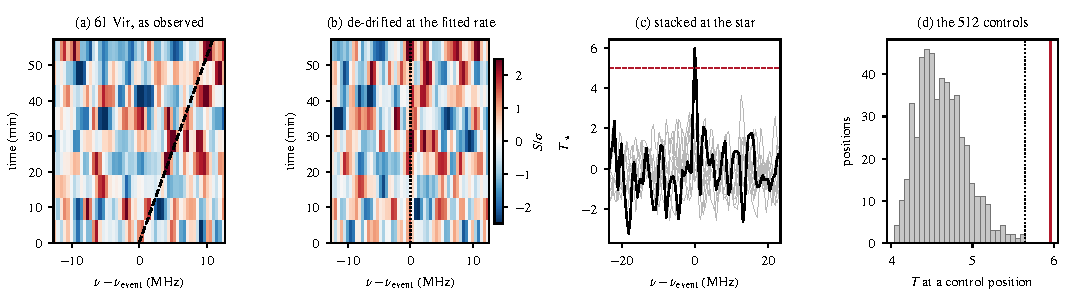
\includegraphics[width=\textwidth]{figures/event_crossings.pdf}
\caption{\textbf{The strongest unattributed crossing of the quality-passing
data, and the control field it leads.} Frequencies are in the star's rest
frame.
\emph{(a)}~The dynamic spectrum at \EvAStar's position around the crossing
at \RqFreqSx\,GHz, observed \EvADate, the fitted drift of
\EvADrift\,Hz\,s$^{-1}$ dashed, \EvANInt{} integrations binned into
\EvANBin{} and plotted in units of each bin's noise.
\emph{(b)}~The same rows shifted by that drift.
\emph{(c)}~The de-drifted stack at the star (black) and at the
\RcNRetCtrl{} control positions with retained dynamic spectra (grey), in
units of its own noise, the trigger dashed. \emph{(d)}~The same statistic at
each of the \NCtrl{} rank-screen control positions: the star (solid) against
the highest control (dotted).}
%% ★ v4.26 (r25-captions): 8 printed lines -> R1 §7's limit of about six.
%% MOVED into \S\ref{sec:vistest} above, carrying seven macros this caption
%% was the only citation site of (\EvAFlux, \EvAFluxErr, \EvARmsInt,
%% \EvAPerIntSig, \EvADwellMin, \EvADriftChan, \EvAChanwkHz,
%% \EvAElapsedMin): the per-integration significance and the drift's reach
%% across the block, both of which are statements about the crossing and not
%% keys to the panels.  DELETED: the closing pointer to
%% Table~\ref{tab:cand} and to \EvBStar{} at \RqFreqCp\,GHz, which
%% \S\ref{sec:vistest}'s own second paragraph states in the same words.
\label{fig:event}
\end{figure*}

\begin{table}
\centering
%% ★★★ v4.26 (r25-captions): 16 PRINTED LINES -> the author's limit.  Nothing
%% here was dropped on the floor: the $\pm\WdHalfKms$ interval and the
%% \TjNCandPair{} it holds are \S\ref{sec:etacrv}'s own second paragraph
%% already; \emph{edge} is defined there verbatim; and the subscript $\star$,
%% the observatory-frame pointer to Appendix~\ref{sec:edge} and the
%% \emph{Miss} column's units are now sentences in that same paragraph, which
%% is where a reader meets the table.  Measured with capmeasure.py.
\caption{\textbf{Can two crossings be one carrier?} The \TjNPair{} pairs
toward one star with an unattributed member. \emph{Miss}, the starred rates,
the control row and the verdicts: \S\ref{sec:etacrv}.}
\label{tab:pairs}
\scriptsize
%% GENERATED by pairs_v415.py -- do not hand-edit.
\begin{tabular}{@{}l@{~}l@{\hspace{4pt}}r@{\,}r@{\,}r@{\,}r@{\hspace{3.5pt}}r@{~}l@{}}
\hline
Star & blocks & $\Delta t$ & $\dot\nu_{1\star}$ & $\dot\nu_{2\star}$ & $\Delta\nu$ & miss & one \\
 & & (d) & \multicolumn{2}{c}{(Hz\,s$^{-1}$)} & (MHz) & ($\sigma$) & carrier? \\
\hline
61~Vir & X822/X82f & 3.00 & $+1092$ & $+3221$ & $+755.4$ & 15 & open \\
J1537$-$3319 & X10359/X398 & 123 & $-2000$ & $+2390$ & $+223.5$ & 3.6 & open \\
AU~Mic & X1838/X319 & 310 & $+1440$ & $+2645$ & $-159.0$ & -- & open \\
HD~14055 & X2b2ee/X2c3bb & 0.09 & $-2390$ & $+4216$ & $+825.2$ & 2447 & no \\
 & X24be0/Xd46 & 1.92 & $+1134$ & $-3823$ & $+63.0$ & 41 & open \\
 & X2c3bb/X3835 & 2.00 & $+4216$ & $+1800$ & $-514.6$ & 144 & edge \\
 & X2b2ee/X3835 & 2.09 & $-2390$ & $+1800$ & $+310.6$ & 48 & open \\
 & X3835/Xd526 & 607 & $+1800$ & $-2563$ & $-555.5$ & -- & open \\
 & X2b2ee/Xd526 & 609 & $-2390$ & $-2563$ & $-244.9$ & -- & open \\
 & X3835/X25c5e & 649 & $+1800$ & $+2611$ & $+423.3$ & -- & open \\
 & X2c3bb/X25c5e & 651 & $+4216$ & $+2611$ & $-91.3$ & -- & edge \\
 & X2b2ee/X25c5e & 651 & $-2390$ & $+2611$ & $+733.8$ & -- & open \\
$\beta$~Pic & X3a90/Xa9df & 1.02 & $-1611$ & $-679$ & $+85.5$ & 132 & open \\
\hline
HD~285968 & X108f/X5b4e & 4.99 & $-29$ & $-29$ & $-0.002$ & 0.6 & yes \\
\hline
\end{tabular}

\end{table}

\begin{table}
\centering
%% ★★★ v4.26 (r25-captions): 15 PRINTED LINES -> the author's limit.  The row
%% stubs of tab_recurcand_v411 already label $T_{\rm pers}$, $T_{\rm rep}$,
%% $(T_{\rm rep}+5)/T_{\rm pers}$ and the $\Phi$ rows in words, so the caption
%% was re-stating the table.  What was NOT anywhere else -- the sign of
%% $T_{\rm rep}$ against the indented maxima, and "in brackets the same at $S$,
%% which is biased high" -- is now \S\ref{sec:vistest}'s prose, two
%% paragraphs above this float.  The half-channel displacement is already in
%% that section ($\pm\RqDispSx$, $\pm\RqDispCp$) and the pointer to
%% Fig.~\ref{fig:event} is already in its first paragraph.
\caption{\textbf{The two events}, the crossings whose
stellar statistic exceeds all \NCtrl{} control positions of their own window.
\S\ref{sec:vistest} reads them.}
\label{tab:cand}
\footnotesize
%% GENERATED by recur_v411.py -- do not hand-edit.
\begin{tabular}{@{}>{\raggedright\arraybackslash}p{0.49\columnwidth}@{~~}r@{~~}r@{}}
\hline
 & 61 Vir & CP$-$72 2713 \\
\hline
Frequency, stellar frame (GHz) & 346.323236 & 344.296455 \\
\quad as delivered, topocentric & 346.313811 & 344.269746 \\
Drift rate (Hz\,s$^{-1}$) & $+3182$ & $-2056$ \\
$T_\star$ & 5.958 & 5.809 \\
Highest control $T$ & 5.65 & 5.68 \\
Fitted amplitude (mJy) & 118.8 $\pm$ 19.9 & 11.3 $\pm$ 2.0 \\
Peak-channel EIRP (W) & $5.1 \times 10^{14}$ & $8.9 \times 10^{14}$ \\
Repeat epochs measured & 3 & 5 \\
\quad of them in the primary census & 3 & 1 \\
\quad census repeats with no retained spectrum & 1 & 0 \\
Nearest covering epoch, separation (h) & $-1.97$ & $+2.05$ \\
\quad covering epochs more than a day away & 2 & 4 \\
Longest baseline (d) & 3 & 2 \\
$T$ expected if persistent, $T_{\rm pers}$ & 9.70 & 6.30 \\
$T$ measured, matched drift, $T_{\rm rep}$ & $+0.39$ & $-0.82$ \\
\quad largest single epoch & $+1.65$ & $+0.96$ \\
\quad maximised over every drift & 2.71 & 3.60 \\
Nearest block alone, $T_{\rm pers}$ & 5.28 & 6.21 \\
\quad $T_{\rm rep}$ & $-0.01$ & $-0.57$ \\
Amplitude still excluded, $(T_{\rm rep}+5)/T_{\rm pers}$ & 0.56 $S$ & 0.66 $S$ \\
\quad from the nearest block alone & 0.95 $S$ & 0.71 $S$ \\
\quad from separated blocks alone & \SpSxFracSep{} $S$ ($n=\SpSxNSep$) & \SpCpFracSep{} $S$ ($n=\SpCpNSep$) \\
\quad over the matched registration tolerance & \SpSxFracTol{} $S$ & \SpCpFracTol{} $S$ \\
Displacement permitted (km\,s$^{-1}$) & $\pm$0.211 & $\pm$0.213 \\
Calculated recovery chance $\Phi$ at $5S/T_\star$ (at $S$) & 1.00 (1.00) & 0.66 (0.90) \\
Disposition & not confirmed & not confirmed \\
\hline
\end{tabular}

\end{table}

%% ★★★★ TABLE 7 (tab:holdout) MOVED TO THE RELEASED FILES, round 25, to
%% the referees' guardrail "Table 7 may move to the catalogue".  It was a
%% full-width float of 0.20 pp carrying a 5-line full-width caption: 0.26 pp
%% in all, measured by floatinv.py and capmeasure.py.
%% ► ITS NAMED HOME, WHICH r25-zenodo MUST PROVIDE: the hold-out crossings as
%%   rows of the crossing ledger, carrying \Delta v_star (the offset from the
%%   nearest masked transition in the star's own frame), n_rep, T_pers, T_rep
%%   and the dagger flag for an offset inside the attribution interval whose
%%   species the attribution set excludes.  Sec. 5.6.2 carries the pointer.
%% ► NOTHING WAS DELETED FROM THE PROSE TO PAY FOR IT: the two readings the
%%   table carried that the text quoted, \HoRecTRep and \HoFracMax, are both
%%   still in Sec. 5.6.2; and the caveat its caption carried -- that a
%%   crossing inside the attribution interval whose species the set excludes
%%   is reported and not acted on -- is stated in Sec. 4.2 and Appendix C, so
%%   it survives exactly once, which is the referees' own rule.
%% ► To restore the float, revert this comment block; tab_holdout_v412.tex is
%%   still generated and still in make_all.sh.

%% tab:ledger MOVED to Appendix D (sections/app_J_falsealarm.tex): a
%% full-width 56-row table* worth 0.72 pp of the main text.  Sec. 5.3 and
%% Sec. 5.6 carry the counts and cite it.



%% fig:chain MOVED to sections/04_method.tex, Sec. 4.2, where it is first
%% cited (referee 2, minor 3).  Sec. 5 cites it at the crossing census.
